\chapter{Implementierung} \label{chap:implementierung}

\section{Backend-Server}

\subsection{Verwendete Technologien}

Die grundlegend verwendete Technologie für den Backend-Server ist die Programmiersprache \enquote{Go}.
Go wurde ausgewählt, da es eine einfach zu verstehende Programmiersprache ist, die optimiert für Server-Anwendungen ist (vgl. \cite{Weigend2019}).
Zudem sind alle am Projekt beteiligten Personen schon mit der Sprache vertraut.

Go stellt eine gute Standardbibliothek zur Verfügung, die an vielen Stellen verwendet wird.
Trotzdem werden zusätzlich einige externe Bibliotheken verwendet.
Diese dienen hauptsächlich dazu, die externen Schnittstellen (\gls{HTTP} und \gls{CoAP}) mit den dazugehörigen Datenformaten zur Verfügung zu stellen.
Auch werden Bibliotheken für ein einfacheres Testing verwendet.

Im Folgenden sind die verwendeten Bibliotheken aufgelistet:
\begin{description}
	\item[logrus (https://github.com/sirupsen/logrus)] \hfill \\
		\enquote{logrus} ist strukturiertes Logging-Tool, dass für jegliche Logs innerhalb des Servers verwendet wird.
	\item[gorm (https://github.com/jinzhu/gorm)] \hfill \\
		\enquote{gorm} ist ein \gls{ORM} Framework, dass die Datenbankanbindung für den Server zur Verfügung stellt.
	\item[Gin (https://github.com/gin-gonic/gin)] \hfill \\
		\enquote{Gin} ist ein HTTP Framework, dass Routing, Parameter-Matching, etc. übernimmt. Zudem kann es standardmäßig \gls{JSON} verstehen.
	\item[go-coap (https://github.com/go-ocf/go-coap)] \hfill \\
		\enquote{go-coap} ist ein \gls{CoAP} Framework, dass hauptsächlich das Routing übernimmt. Einige weitere Aufgaben, die z.B. \enquote{Gin} übernimmt, müssen selbst programmiert werden.
	\item[go-codec (https://github.com/ugorji/go)] \hfill \\
		\enquote{go-codec} stellt die Codierung für \gls{CBOR} zur Verfügung.
	\item[now (https://github.com/jinzhu/now)] \hfill \\
		\enquote{now} stellt Hilfsfunktionen zur Verfügung für Zeitberechnungen.
	\item[xlsx (https://github.com/tealeg/xlsx)] \hfill \\
		Mit \enquote{xlsx} können Dateien im \gls{XLSX} Dateiformat erstellt, bearbeitet und gelesen werden. Im Server wird sie für das Erstellen des Excel-Export genutzt.
	\item[ginkgo (https://github.com/onsi/ginkgo)] \hfill \\
		Mit \enquote{ginkgo} können Tests in \gls{BDD} Technik geschrieben werden.
	\item[gomega (https://github.com/onsi/gomega)] \hfill \\
		\enquote{gomega} ist eine Matching Library, die zu \enquote{ginkgo} gehört. Sie stellt Vergleiche zwischen erwarteten Werten und tatsächlichen Werten zur Verfügung.
	\item[GoMock (https://github.com/golang/mock)] \hfill \\
		\enquote{GoMock} ist ein Mocking Framework, dass für verschiedene Tests verwendet wird.
\end{description}

Als Datenbank wird in Kombination mit \enquote{gorm} eine \enquote{SQLite} verwendet.
Der große Vorteil ist, dass eine SQLite Datenbank eine einfache Datei ist und kein externer Server aufgesetzt werden muss.
Dies vereinfacht vor allem die Entwicklung.
Zum Beispiel ist ein einfaches Zurücksetzten der Daten durch ein Löschen der Datei möglich.

In einem späteren Einsatz des Paper-Trackers kann dank der \enquote{gorm} Bibliothek auch andere Datenbanken verwendet werden, die eher für einen dauerhaften und sichereren Einsatz vorgesehen sind.
Möglich sind dafür \enquote{MySQL}, \enquote{PostgreSQL}, \enquote{Microsoft SQL Server} und wie erwähnt SQLite.
Im Code des Servers muss hierfür lediglich eine erweiterte Konfiguration ermöglicht werden. (vgl. \cite{Jinzhu2020})

\subsection{REST-Schnittstelle}

\subsection{CoAP-Schnittstelle}

\subsection{Tracker-Lokalisierung}

Wie in \autoref{sec:tracking-hardware} beschrieben wird die Lokalisierung der Tracker mit einem
Score-basierten Sysytem durchgeführt.

Dazu werden zunächst Scanergebnisse vom jeweiligen Tracker gesammelt und dann ausgewertet. Da die
Datengröße der Scanergebnisse je nach Anzahl der vom Tracker sichtbaren \gls{WLAN}-Netzwerken zu
groß für ein einzelnes \gls{UDP}-Paket ist\footnote{Im Arduino-Framework gibt es eine
Limitierung von 1446 Bytes für die Größe eines \gls{UDP}-Paketes. (vgl. \cite{Arduino2020})}, wurde
das \gls{API} so gestaltet, dass die Ergebnisse in mehreren Paketen an den Server übermittelt werden
können. Dazu berechnet der Tracker im Vorraus, in wie viele Pakete die Scanergebnisse geteilt werden
müssen. Diese Zahl, sowie ein für den Ergebnissatz einheitlicher, zufällig erzeugter \gls{ID} sind
jedem Teilpaket angehängt. So kann der Server erkennen, ob alle Ergebnisse empfangen wurden und
diese dann verwenden. Dass nicht alle Pakete eines Ergebnissatzes beim Server angekommen sind ist
dadurch erkennbar, dass ein anderer \gls{ID} empfangen wird. In diesem Fall werden alle vom
vorherigen Paket empfangenen Scanergebnisse verworfen und die neuen Pakete gespeichert.
\TODO{Das hier kann vielleicht zu CoAP-Schnittstelle verschoben werden}

Sobald ein vollständiger Ergebnissatz empfangen wurde, wir aus diesem ein Score für jeden Raum
ermittelt. Dieser Score ist eine positive Ganzzahl
\section{Hardware und Firmware}

Im Folgenden wird erläutert, wie der Tracker hinsichtlich der verwendeten Hardware und der
entsprechenden Firmware implementiert wurde.

\subsection{Verwendete Technologien}

Als Mikrokontrollerplattform wurde die sogenannte \enquote{TinyPICO}-Plattform gewählt. Nach eigener
Aussage handelt es sich dabei um die kleinste vorgefertigte Entwicklungsplattform basierend auf
Mikrocontrollern vom Typ ESP32. Dieser Aspekt ist für die Erfüllung von \ref{nf:klein} wichtig.
Dieser Mikrocontroller wurde gewählt, da er alle benötigten Funktionen wie beispielsweise \gls{WLAN}
bereits über ein \gls{API} bereitstellt.

Die TinyPICO-Entwicklungsplattform stellt neben dem Mikrocontroller weitere Hardware bereit, so sind
unter anderem
die Stromversorgung über \gls{USB} sowie Lithium-Polymer-\gls{Akku}, ein Übersetzer von \gls{USB}
zu \gls{UART} zur Programmierung des Mikrocontroller und eine Vollspektrum-\gls{LED} verbaut.
Ein weiterer Vorteil ist das bereits integrierte Ladesystem, welches einen angeschlossen
Lithium-Polymer-\gls{Akku} automatisch auflädt, sobald der Tracker über \gls{USB} mit einer
Stromquelle verbunden wird. Außerdem können über das Ladesystem der aktuelle Ladezustand und die
Spannung des \gls{Akku} abgefragt werden, was für die Erfüllung von \ref{fa:benachrichtigung}
unabdingbar ist.

Die Firmware wurde in der Programmiersprache C++ auf Basis des Arduino-Frameworks erstellt. Dieses
Framework wurde gewählt, da es auf vielen Plattformen, wie auch dem ESP32 lauffähig ist, weit
verbreitet ist und somit viele Bibliotheken für das Framework existieren.

Das \enquote{Flasher}-Tool zum Programmieren und Konfigurieren der Firmware wurde in Python
entwickelt.
Der Grund dafür liegt in Möglichkeit sehr schnell und simpel ein Programm und auch ein \gls{GUI} zu
programmieren.
Dies wird durch die Bibliothek \enquote{PySimpleGUI} ermöglicht, die lediglich mit einer groben Layout-Beschreibung
ein Oberfläche zusammenstellt.
Alle weiteren benötigten Bibliotheken sind in der Python-Standardbibliothek enthalten.
Vor allem ist hierbei die \enquote{multiprocessing}-Bibliothek wichtig, mit welcher andere Programme aufgerufen werden können.
Um aus dem enstandenen Python-Skript eine ausführbare Datei für die verbreitesten Betriebssysteme zu erstellen, wird \enquote{PyInstaller} verwendet.
Die daraus enstehende Datei beinhaltet bis auf das PlatformIO-Tooling alle benötigten Ressourcen. \TODO{Kann man das mit bundeln?!}

\subsection{Flasher}
Aufgrund der angestrebten Einfachheit dieses Programmes, besteht es aus insgesamt nur drei Dateien.
Der Hauptbestandteil des Flashers ist das eigentliche Python-Skript.
Zusätzlich wird die Datei \enquote{requirements.txt} benötigt, welche alle Bibliotheken für den
Bibliotheksmanager \enquote{pip} auflistet.
In dieser Datei sind lediglich, wie oben erwähnt, \enquote{pysimplegui} und \enquote{pyinstaller} aufgeführt.
Die dritte und letzte Datei ist ein \enquote{Makefile}, welches einige Befehle zum Installieren der Bibliotheken,
Ausführen des Skripts oder Erstellen der ausführbaren Datei bereitstellt.

Das Skript selbst beginnt nach dem Importieren der benötigten Bibliotheken mit dem Parsen der
Kommandozeilenargumente.
Möglich ist nur das Argument \texttt{--keep-credentials}.
Das Skript erzeugt eine Datei, in welcher die Zugangsdaten für das vom Tracker zu verwendende
\gls{WLAN}-Netzwerk, sowie weitere potentiell sensitiven Informationen enthalten sind. Im
Standardfall wird diese Datei nach dem Erstelln der Firmware und der Programmierung des Trackers
gelöscht. Ist das Kommandozeilenargument \texttt{--keep-credentials} gegeben, wir die Datei nach
Erfolgreichem Abschluss des Programmiervorganges nicht gelöscht, was vor allem in der
Entwicklungsphase der Software vorteilhaft ist.

Weiter werden einige Konstanten definiert.
Diese sind zum einen der Titel des Programm-Fensters und einige sogenannte \enquote{Keys},
die eindeutig bestimmte Elemente der \gls{GUI} identifizieren.

Nach den Konstanten werden drei Funktionen definiert, die die eigentliche Logik des Flashers beinhalten.
Zuerst eine Funktion, die alle möglichen Ports, über die ein Tracker programmiert werden kann, auflistet.
Dies wird über ein Aufrufen von PlatformIO ermöglicht: \enquote{pio device list}.

Die nächste Funktion generiert die für die Firmware benötigte Datei mit der Konfiguration des Trackers.
Sie liest ein Template mit Platzhalter-Werten der Datei ein und ersetzt die Platzhalter mit den eingegebenen Werten, die als Parameter übergeben werden.
Nach dem Einsetzen der Werte, wird die Datei geschrieben.
Der Pfad, an dem sich die Firmware befindet, ist auch Teil der Werte, die als Parameter übergeben werden.
Zugriff auf einen einzelnen Wert wird über die oben erwähnten konstanten \enquote{Keys} ermöglicht.

In der letzten Funktion wird das Programmieren an sich ausgeführt.
Auch diese Funktion bekommt die eingebenene Werte als Parameter. Aus diesen wird der ausgewählte Port benötigt.
Mit diesem wird wieder PlatformIO aufgerufen: \enquote{pio run -e tinypico -t upload --upload-port port}.

Vor dem Hauptteil des Skripts werden noch die Layouts für die \gls{GUI} benötigt.
Es werden zwei verschiedene Layouts definiert: Ein Eingabe-Layout und ein Programmier-Layout.
Das Eingabe-Layout ist in \autoref{fig:flasher-input} dargestellt.
Es ist eine Tabelle aus Eingabe-Feldern mit Erklärungen, in denen alle benötigten Konfigurationen eingetragen werden können.
Die Eingabe-Felder selbst sind mit den Keys verknüpft.
Am unteren Teil des Layouts befindet sich ein Button, der das Programmieren startet.

\begin{figure}
	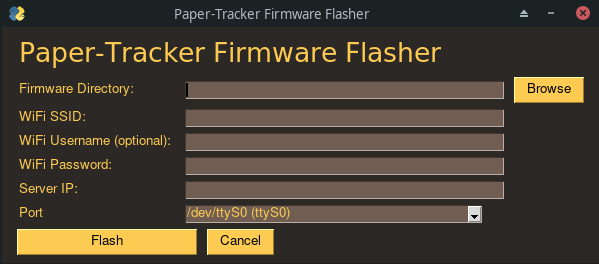
\includegraphics[width=\textwidth]{images/flasher/input.png}
	\centering
	\caption{Layout des Eingabe-Fenster}
	\label{fig:flasher-input}
\end{figure}

Das Programmier-Layout besteht lediglich aus einem Titel, einem Textfeld und einem Button.
Es ist in \autoref{fig:flasher-flash} dargestellt.
Im Textfeld soll der aktuelle Status angezeigt werden.
Der Button ist zum Schließen des Programms, sobald der Vorgang abgeschlossen ist.

\begin{figure}
	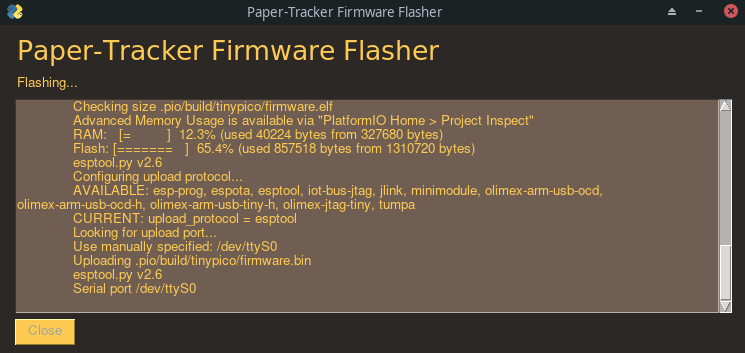
\includegraphics[width=\textwidth]{images/flasher/flash.png}
	\centering
	\caption{Layout des Programmier-Fenster}
	\label{fig:flasher-flash}
\end{figure}

Im Hauptteil des Skripts werden nun zuerst das Fenster mit dem Eingabe-Layout geöffnet.
Sobald der Button zum Start gedrückt wurde, werden die eingegebenen Werte ausgelesen.
Das Eingabe-Fenster wird geschlossen und das Programmier-Fenster mit den entsprechendem Layout geöffnet.
Ist dieses offen, wird die Funktion zum Generieren der Konfigurationsdatei und die Funktion zum Programmieren des Trackers aufgerufen.
Im Textfeld des Layouts werden diese Schritte entsprechend dokumentiert.
Auch die Ausgabe des Programmierens wird in das Textfeld ausgegeben.
Nach dem Programmieren wird, je nach Kommandozeilenargument, die generierte Datei gelöscht.
Nun kann das Fenster und damit das gesamte Programm über den Schließen-Button geschlossen werden.

Tritt während diesem gesamten Vorgang ein Fehler auf, wird dieser entsprechend aufgefangen und die Fehlermeldung im Textfeld angezeigt.
Das Löschen der generierten Datei wird auf im Fehlerfall ausgeführt.

\section{App}

Im diesem Kapitel wird die technische Umsetzung der App für Mobilgeräte beschrieben.

\subsection{Verwendete Technologien}

Zur Programmierung der App wurden die Programmiersprache Dart und das Framework Flutter verwendet.
Ein großer Vorteil dieser Kombination ist, dass Anwendungen sowohl für Android, als auch für iOS
kompiliert werden können, ohne den Quellcode anpassen zu müssen. Auch eine Laufzeitumgebung für
Desktopcomputer unter Windows, macOS und GNU/Linux befindet sich aktuell im Teststadium, sodass die
Paper-Tracker App gegebenenfalles auch auf Arbeitsplatzrechnern verwendet werden kann.

Auch für das Erstellen der App wurden einige Bibliotheken verwendet, die die Entwicklung vereinfachen.
Vor allem werden zum Beispiel Bibliotheken verwendet, um die Kommunikation mit dem Backend-Server zu ermöglichen.
Die verwendeten Bibliotheken sind im Folgenden aufgelistet:
\begin{description}
	\item[http (https://pub.dev/packages/http)] \hfill \\
		\enquote{http} ist eine Bilbiothek, die es ermöglicht asynchron \gls{HTTP}-Anfragen durchzuführen. Die Bibliothek wird dafür verwendet, um mit dem Backend-Server zu kommunizieren.
	\item[json\_annotation (https://pub.dev/packages/json\_annotation)] \hfill \\
		Mit \enquote{json\_annotation} kann über Annotationen im Programmcode eine Serialisierung zu JSON und Deserialisierung von JSON für Datenklassen generiert werden.
	\item[shared\_preferences (https://pub.dev/packages/shared\_preferences)] \hfill \\
		Durch die \enquote{shared\_preferences} Bibliothek können einfache Konfigurationen als Schlüssel-Wert-Paare abgespeichert werden. Dies wird für die \gls{URL} des Backend-Servers verwendet.
	\item[material\_design\_icons (https://pub.dev/packages/material\_design\_icons\_flutter)] \hfill \\
		\enquote{material\_design\_icons} stellt zusätzliche Material\footnote{Eine Designsprache von
			Google, die in fast allen Google-Produkten eingesetzt wird und auf Minimalismus setzt.
			\cite{Google2020}}-Icons zur Verfügung. Dies ist notwendig, da die standardmäßig verfügbaren Icons in Flutter nicht ausreichend sind.
	\item[fluttertoast (https://pub.dev/packages/fluttertoast)] \hfill \\
		Mit \enquote{fluttertoast} können kleine Pop-ups dargestellt werden, die dem Nutzer der App einfach und schnell Feedback zu einer Aktion geben können.
\end{description}

\section{Bestehende Herausforderungen}
% Erstmal ein paar Beispiele
\subsection{Ungenauigkeit des Tracking}

\subsection{UI-Details in der App}
